\chapter{Metodología}
\label{ch:metodologia}

A lo largo de este capítulo señalaremos con qué métodos y herramientas lograremos, con éxito, el objetivo de este trabajo. Estas estarán basadas en la experiencia de trabajos previos revisados en el Capitulo~\ref{ch:marcoteorico} y metodologías ampliamente utilizadas en la minería de datos [cita] para la obtención de información valiosa en los datos de forma efectiva.

\section{Minería de Datos}
La cantidad de datos ha ido aumentando de forma exponencial debido a los avances en la tecnología de la computación necesitando que la búsqueda de conocimiento sea de forma automatizada.
La minería de datos es un proceso que se ideó pensando en descubrir información valiosa dentro de una gran cantidad de datos\footnote{Para este trabajo definimos datos como información textual o numérica con alguna estructura dada} como flujo de entrada y nos entrega conocimiento.\footnote{Esto es una analogía a la industria de la minería donde se extrae los minerales rocosos donde una parte de esta es valiosa}

[grafico]
http://storm.cis.fordham.edu/~gweiss/papers/data-mining-chapter-2010.pdf

La minería de datos tiene como finalidad obtener información valiosa para la toma de decisiones o para la comprensión de un fenómeno y se realiza a través de diferentes tareas que se pueden realizar con los diferentes algoritmos disponibles que los señalaremos posteriormente.

Para realizar la minería de datos se han establecido diferentes metodologías para asegurar un resultado coherente con lo que se busca obtener. Existen diferentes metodologías que serán mencionadas y descritas brevemente a continuación.

\subsubsection{KDD}
[cita] http://www.csd.uwo.ca/faculty/ling/cs435/fayyad.pdf
La metodología \textit{Knowledge Discovery in Databases} o Proceso de Extracción del Conocimiento, tal como su nombre lo dice, es un proceso no trivial de descubrimiento de conocimiento e información potencialmente útil dentro de los datos contenidos en algún repositorio de información (cita de Han, J.; Kamber M. (2001). Data Mining: Concepts ans Techniques. Morgan Kaufmann Publishers, USA.). 

Es un proceso iterativo que explora de forma exhaustiva altos volúmenes de datos con el fin de determinar relaciones. De esta manera es posible extraer información de calidad que se puede utilizar para generar modelos con los datos. 

\begin{figure}[H]
  \centering
    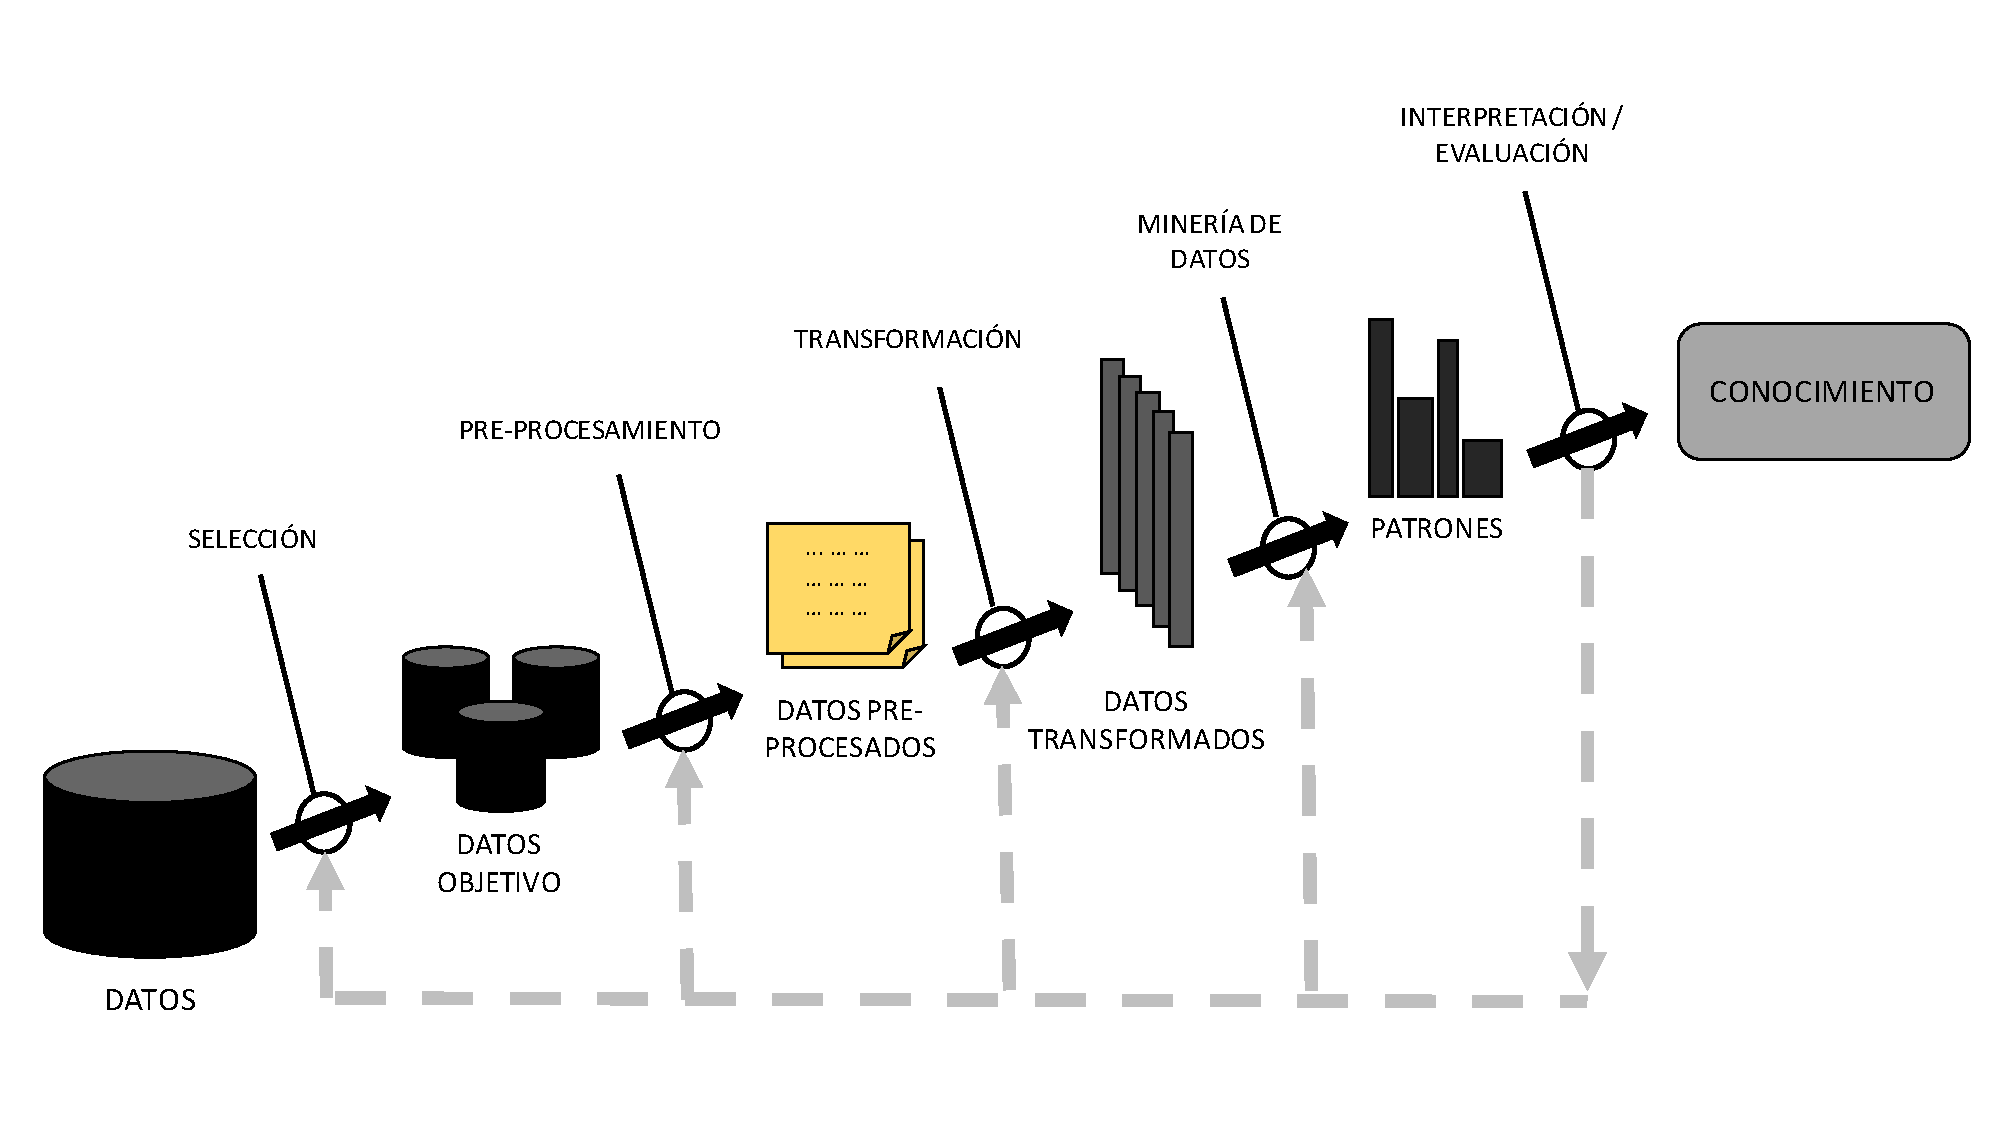
\includegraphics[width=0.9\textwidth]{Figuras/KDD}
      \caption{Etapas de la metodología KDD.}
    \label{fig:kdd}
\end{figure}

Como muestra la Figura~\ref{fig:kdd}, el proceso de extracción del conocimiento consta de cinco etapas:
\begin{description}
  \item[1. Selección de Datos:] se determinan las fuentes de datos y el tipo de información a utilizar, es cuando los datos relevantes para el análisis son extraídos de la o las fuentes de datos.
  \item[2. Pre-Procesamiento:] se procede a preparar y limpiar los datos extraídos desde las distintas fuentes de datos seleccionadas anteriormente. Este paso es fundamental para las fases posteriores.Para manejar datos faltantes, inconsistentes o que estén fuera de rango se utilizan diversas estrategias con el fin de obtener una estructura de datos adecuada para su posterior transformación.
  \item[3. Transformación:] consiste en el tratamiento preliminar de los datos, transformando y generando nuevas variables con una estructura de datos apropiada a partir de las ya existentes. Se realizan operaciones de agregación o normalización, consolidando los datos de una forma necesaria para la fase siguiente. 
  \item[4. Minería de Datos:] consiste en el modelamiento propiamente tal, para lo que se aplican métodos inteligentes con el fin de extraer patrones desconocidos, válidos, nuevos, potencialmente útiles y comprensibles y que están "ocultos" en los datos.
  \item[5. Interpretación y Evaluación:] finalmente se identifican los patrones obtenidos y que son realmente interesantes, además de evaluar los resultados obtenidos.
\end{description}

\subsubsection{SEMMA}
La metodología SEMMA, acrónimo de \textit{Sample, Explore, Modify, Model, Assess}, se define como un proceso de selección, exploración y modelamiento de grandes cantidades de datos para descubrir patrones de negocios desconocidos. 

\begin{figure}[H]
  \centering
    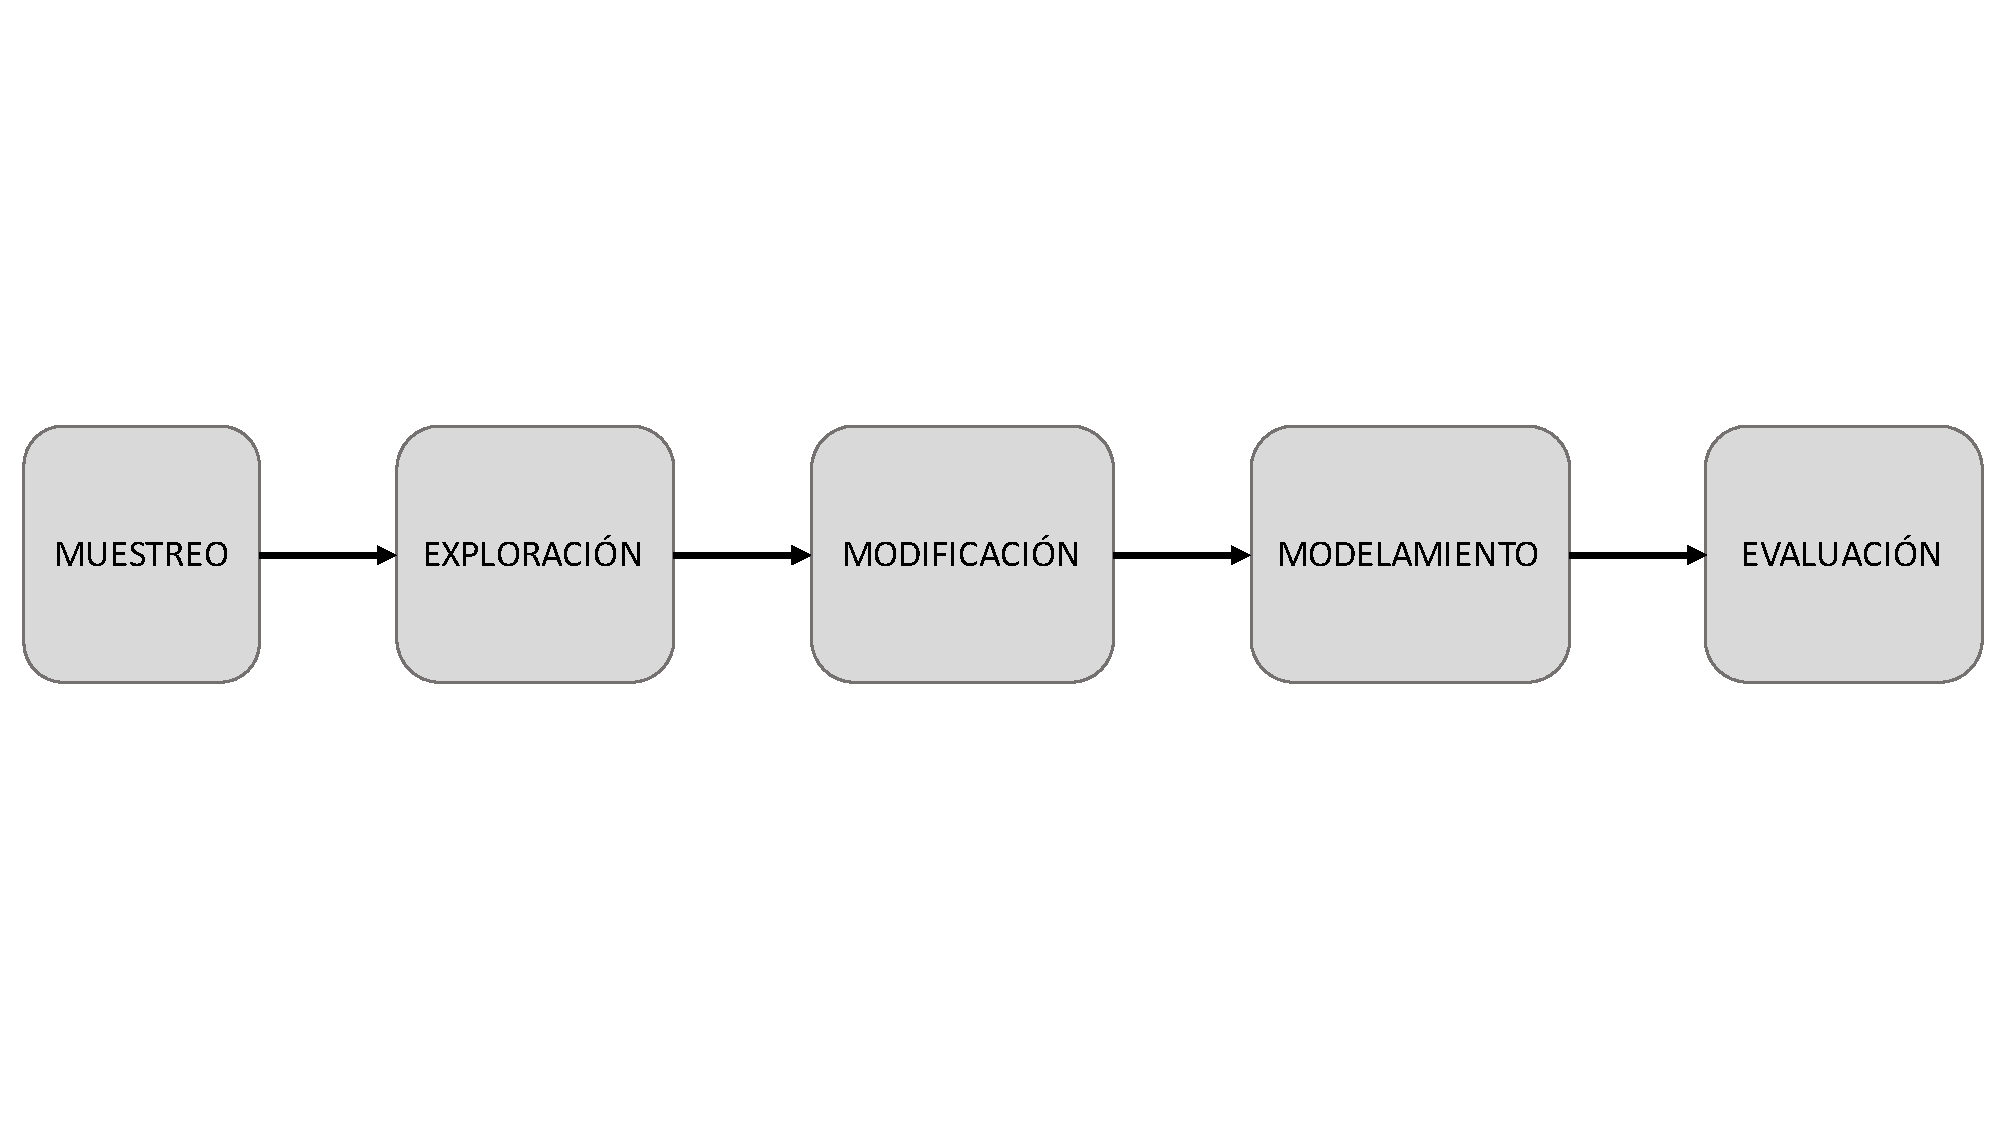
\includegraphics[width=0.9\textwidth]{Figuras/SEMMA}
      \caption{Etapas de la metodología SEMMA.}
    \label{fig:semma}
\end{figure}

En la Figura~\ref{fig:semma} es posible observar que esta metodología consta de cinco etapas:
\begin{description}
  \item[1. Muestreo:] es la etapa inicial, en la cual se procede a preparar los datos para su posterior exploración. En esta etapa es común la utilización del nodo de partición (especialmente si se quiere realizar árboles de decisión o redes neuronales). 
  \item[2. Exploración:] en esta etapa, como lo dice su nombre, se procede a explorar los datos, por lo que es una de las más trabajosas. Se tiene un nodo que permite explorar gráficamente los datos y otro de selección de variables que permite eliminar aquellos datos de entrada que no tienen relación con la variable objetivo, inclusive se puede realizar un análisis de conglomerados o una segmentación.
  \item[3. Modificación:] en esta etapa el foco es la selección y transformación de variables y datos que servirán para la posterior construcción de modelos. Entre otras tareas, destaca la reducción de dimensión y la imputación de datos perdidos o anómalos.
  \item[4. Modelamiento:] en esta etapa se procede a la selección de modelos. Esta elección depende esencialmente de los datos y variables que se tienen, y de obtener modelos fácilmente entendibles. Entre los modelos está la regresión, la regresión logística, árboles de decisión, análisis factorial discriminante, redes neuronales, entre otros. Se puede aplicar más de uno a la vez, para luego comparar los resultados obtenidos.
  \item[5. Evaluación:] etapa final en la cual se procede a comparar los modelos aplicados y los resultados que se obtienen de ellos. 
\end{description}
[cita]

\subsubsection{CRISP-DM}
La metodología CRISP-DM o \textit{Cross-Industry Standard Process for Data Mining} es un estándar para los proyectos de minería de datos que incluye un modelo y una guía, estructurados en fases que pueden ser bidireccionales, es decir, al desarrollar una fase es posible revisar parcial o totalmente las anteriores. 

\begin{figure}[H]
  \centering
    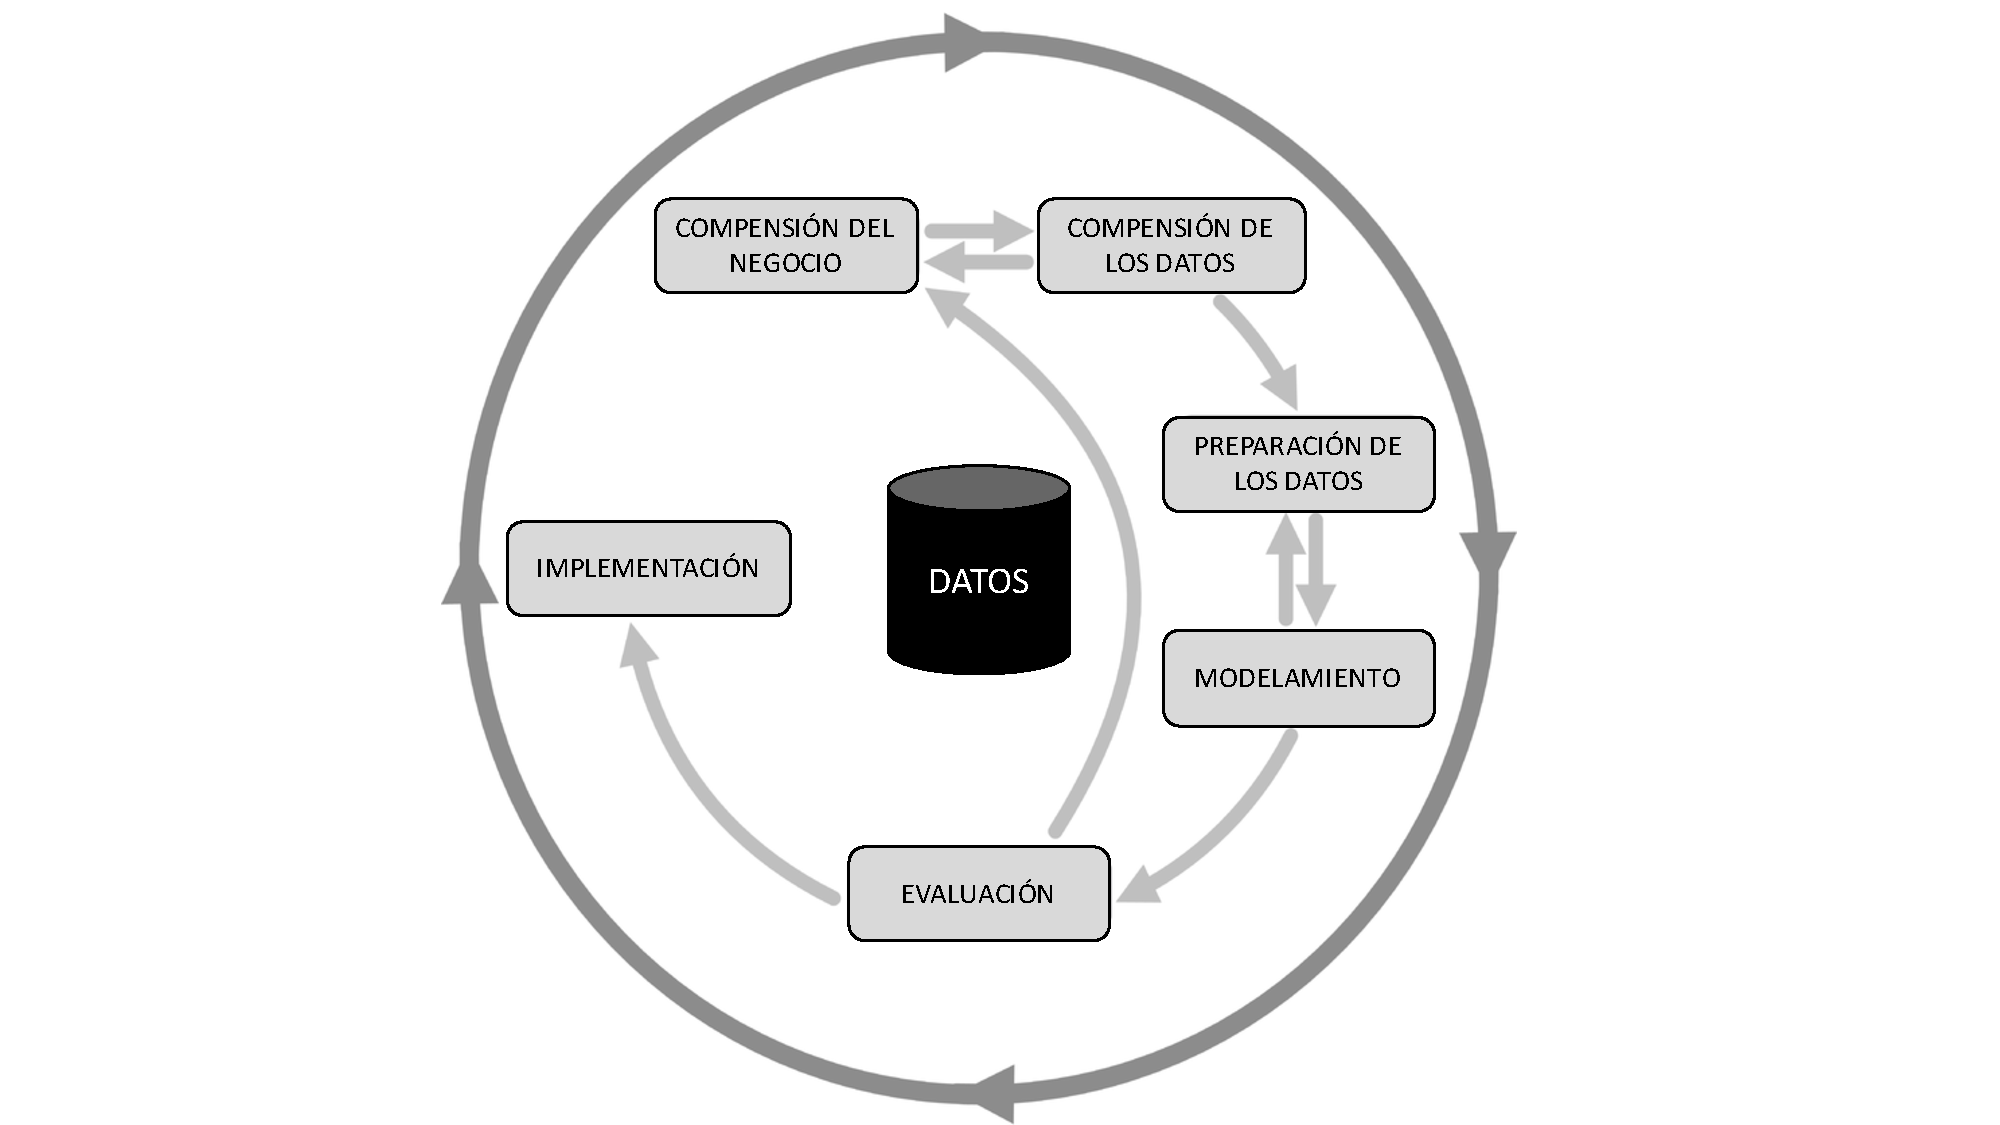
\includegraphics[width=0.99\textwidth]{Figuras/CRISP}
      \caption{Etapas de la metodología CRISP-DM.}
    \label{fig:crisp}
\end{figure}

Como es posible observar en la Figura~\ref{fig:crisp}, esta metodología estructura el proceso en seis fases cuya sucesión no es necesariamente rígida. Cada fase se descompone en varias tareas generales de segundo nivel. Las tareas generales se proyectan a tareas específicas, pero en ningún momento se propone como realizarlas. Es decir, CRISP-DM establece un conjunto de tareas y actividades para cada fase del proyecto pero no especifica cómo llevarlas a cabo.

Las fases son: 
\begin{description}
  \item[1. Comprensión del Negocio:] fase inicial cuyo objetivo es la comprensión de los objetivos y requisitos del cliente, para luego convertir este conocimiento en objetivos técnicos y en un plan de proyecto. 
  \item[2. Comprensión de los Datos:] el objetivo es establecer un primer contacto con el problema, por lo que requiere una recolección inicial de datos para familiarizarse con ellos, identificar su calidad y establecer las relaciones más evidentes para luego definir las primeras hipótesis. Esta fase junto a las próximas dos, son las que demandan el mayor esfuerzo y tiempo en un proyecto de minería de datos.
  \item[3. Preparación de los Datos:] una vez efectuada la recolección inicial de datos, se procede a su preparación para adaptarlos a las técnicas de minería de datos que posteriormente se utilicen. Este proceso incluye tareas generales de selección de datos a los que se va a aplicar una determinada técnica de modelado, limpieza de datos, generación de variables adicionales, integración de diferentes orígenes de datos y cambios de formato.
  \item[4. Modelamiento:] se seleccionan las técnicas de modelado apropiadas para el proyecto. Esta selección se debe realizar en función de los siguientes criterios: que sea apropiada al problema, disponer de los datos adecuados, cumplir con los requisitos del problema, tiempo adecuado para obtener un modelo y conocimiento de la técnica. 
  \item[5. Evaluación:] se procede a la evaluación del modelo considerando el cumplimiento de los criterios de éxito del problema. Además, debe considerarse que la fiabilidad calculada para el modelo se aplique sólo para los datos sobre los que se realizó el análisis. Es preciso revisar el proceso, teniendo en cuenta los resultados obtenidos, para poder repetir algún paso anterior, en el que se haya posiblemente cometido algún error. Es importante considerar que se pueden emplear múltiples herramientas para la interpretación de los resultados. Luego, si el modelo generado es válido en función de los criterios de éxito establecidos en la fase anterior, se procede a la explotación del modelo.
  \item[6. Implementación:] luego de que el modelo ha sido construido y validado, se procede a transformar el conocimiento obtenido en acciones dentro del proceso de negocio.
\end{description}

[cita] http://oldemarrodriguez.com/yahoo_site_admin/assets/docs/Documento_CRISP-DM.2385037.pdf

Para poder cumplir con los objetivos del trabajo debemos seleccionar una metodología de minería de datos. Los estudios muestran que la metodología CRISP-DM es la más simple y a la vez completa, abarcando desde el entendimiento del negocio hasta la implementación de la herramienta de minería de datos.[cita]A Comparative Study of Data Mining Process Models (KDD, CRISP-DM and SEMMA) Además, se ha visto durante varios años que la metodología CRISP-DM es la más utilizada dentro de la comunidad [cita] http://www.kdnuggets.com/2014/10/crisp-dm-top-methodology-analytics-data-mining-data-science-projects.html

[tabla] Table 1: Summary of KDD, CRISP-DM and SEMMA Processes [cita] A Comparative Study of Data Mining Process Models (KDD, CRISP-DM and SEMMA) 

En base a lo anterior, para desarrollar el trabajo se utilizará la metodología CRISP-DM.

\subsection{Utilidad}
\subsubsection{Clasificación y Regresión}
La clasificación y regresión involucra la predicción de una variable específica a través de un modelo de dependencia de otras variables. La diferencia entre la clasificación y la regresión, es que la primera tiene como variable objetivo del tipo discreta y la segunda de carácter continua. Ejemplos de clasificación se ven en problema de detección de transacciones de tarjetas de crédito fraudulentas y ejemplos de regresión se pueden ver en predicción del precio de una acción hasta la planificación de producción de una empresa.[cita] http://storm.cis.fordham.edu/~gweiss/papers/data-mining-chapter-2010.pdf

Matemáticamente podemos ver lo siguiente:\\
Teniendo $N$ observaciones con variables $x_1, x_2, x_3, ... , x_i$ se busca predecir el valor de las variables $y_1, y_2, y_3, ... , y_j$ para las $N$ observaciones de forma independiente.
Utilizando algoritmos de aprendizaje automatizado se busca encontrar una función tal que
$f(x_1, x_2, x_3, ... , x_i) = y_1, y_2, y_3, ... , y_j$
[grafico]
\subsubsection{Análisis de Reglas Asociativas}
El analisis de reglas asociativas busca descubrir patrones o asociaciones en base a diferentes elementos en un conjunto de datos. El más comun de este analisis es el analisis de los carritos de compras en un supermercado. Lo que se busca en este caso es buscar el patrón de compras conjuntas, por ejemplo se puede encontrar un patrón común $\{\textrm{Hamburguesa, Pan}\} \to \textrm{Ketchup}$, es decir, en general las personas que llevan hamburguesa y pan de hamburguesa en el carrito de compra, es probable que también lleven ketchup.[grafico]*

\subsubsection{Análisis de Conglomerados}
Este análisis tiene como objetivo agrupar variables similares en un mismo conglomerado. Las aplicaciones de esto pueden ser la agrupación de documentos de noticias en base al uso de un buscador.

Matemáticamente podemos ver lo siguiente:\\
Teniendo $N$ observaciones con variables $x_1, x_2, x_3, ... , x_i$ se buscan agrupar estas variables en $M$ conglomerados en base a las $N$ observaciones de cada variable. Este método se puede aplicar tanto como a las observaciones o variables.
[grafico]

[revisar] http://eprints.iisc.ernet.in/273/1/p264-jain.pdf

\subsection{Transformación de los Datos}
La transformación de datos debe estar presente cuando se quiere aplicar minería de datos, ya que es un paso fundamental para que los datos sean legibles y válidos para los algoritmos del procedimiento del modelamiento.

Los procedimientos utilizados en esta etapa son los siguientes:

\begin{description}
  \item[Agrupación de Datos]
  Cuando se tiene muchos datos a veces resulta útil agruparlos para lograr una reducción de estos mejorando su calidad.
  \item[Estructuración de Datos]
  Hay veces donde los datos no  vienen estructurados de la misma forma o simplemente no hay estructura dada. para poder realizar un trabajo de minería de datos es necesario tener un estándar en la estructura de los datos. Por ejemplo, cuando se obtiene información de una página web, esta generalmente no posee una estructura dada, sino que, hay que crearle una para que sea legible y si se tienen más fuentes de datos, es necesario unificar la estructura en una sola.
  \item[Normalización y Discretización de Datos]
  Para que el modelamiento entregue resultados coherentes con la realidad, es sumamente necesario normalizar, discretizar y vectorizar los datos.\\
  La normalización es un procedimiento donde se modifica la escala de los datos logrando que todos tengan una escala de magnitudes similares donde la distancia representará la información y no la magnitud. Generalmente se normaliza utilizando el siguiente procedimiento matemático:
  [formula]
  
  Otra forma de normalizar, que más bien se habla de escalamiento, es utilizando una escala uniforme establecimiento el mínimo y el máximo en la escala. Matemáticamente se puede ver lo siguiente:
  [formula]
  
  Finalmente la discretización y vectorización de los datos implica el uso de algoritmos que son capaces de manejar datos que no poseen magnitud, es decir, categorías para transformarlos en algo númerico que sea legible para el modelo.
  
  La discretización es un procedimiento que lo hace es asignarle números a las categorías, es decir, si tenemos una variable que contiene las siguientes categorias $\{\textrm{Santiago, La Florida, Lo Espejo}\}$ el algoritmo transformará está información en $\{1,2,3\}$. 
  
  La vectorización es también un procedimiento para transformar categorías, pero es aún más util, puesto que separa cada categoría en una nueva variable donde se señala si se presenta o no cierta categoria. Utilizando el ejemplo anterior donde tenemos una variable categorica con las siguientes categorias $\{\textrm{Santiago, La Florida, Lo Espejo}\}$, al realizar la vectorización, el algortimo como se puede ver en la Figura~\ref{fig:vect} crea 3 variables dónde cada una indica si la observación es de Santiago, La Florida ó Lo Espejo de forma separada, dónde $1$ señala que presenta esa caracteristica y $0$ cuando no la presenta.
    \begin{table}[H]
    \centering
    \begin{tabular}{l|c|c|c|}
    \cline{2-4}
     & \multicolumn{1}{l|}{\textbf{SANTIAGO}} & \multicolumn{1}{l|}{\textbf{LA FLORIDA}} & \multicolumn{1}{l|}{\textbf{LO ESPEJO}} \\ \hline
    \multicolumn{1}{|l|}{Observación 1} & \textbf{1} & 0 & 0 \\ \hline
    \multicolumn{1}{|l|}{Observación 2} & 0 & \textbf{1} & 0 \\ \hline
    \multicolumn{1}{|l|}{Observación 3} & 0 & 0 & \textbf{1} \\ \hline
    \end{tabular}
    \caption{Ejemplo de una vectorización de variables categóricas}
    \label{fig:vect}
    \end{table}
      
  Todo esto se utiliza por que normalmente los algoritmos de aprendizaje automático requieren el uso de variables númericas donde la distancia entre los datos es la que se compara, por tanto, no tendría sentido utilizar variables categoricas de texto ni tampoco usar dos variables que tengan diferentes escalas, puesto que los resultados entregados por este estarían influenciados por la variable que tenga la escala más grande.\footnote{Existen métodos que automáticamente manejan estos conflictos. Se hablará de estos más adelante.}

\end{description}


\\ La importancia de este proceso se puede resumir en tres puntos:

\begin{enumerate}
  \item Los datos se obtienen del mundo real donde puede estar incompleta, con ruido y ser inconsistente
  \item La preparación de datos genera un conjunto de datos más pequeño que el original logrando menos tiempo de procesamiento en el proceso del modelamiento
  \item La preparación de datos genera conjuntos de datos de calidad mejorando los patrones encontrados
\end{enumerate}
[cita] http://www.cs.ccsu.edu/~markov/ccsu_courses/datamining-3.html
\subsection{Algoritmos de Aprendizaje Automatizado}

\subsection{Validación de los Resultados}

\section{Herramientas Computacionales}
Para poder desarrollar este trabajo se deben integrar diferentes herramientas para realizar la transformación, preparación, modelamiento y validación de los datos.
\subsection{Lenguaje de Programación Python}
Python es un lenguaje de programación de alto nivel para resolver todo tipo de problemas. Este soporta programar en diferentes paradigmas y manejo automático del uso de recursos. Además tiene un énfasis en la legibilidad imponiendo un orden en el código.
En general, las ventajas de Python son las siguientes:\\
\begin{itemize}
  \item Intuitivo
  \item Flexible
  \item Comunidad activa
  \item Excelente documentación
\end{itemize}
Python se basa en paquetes o librerías para poder distribuir soluciones especificas, a continuación se nombrarán las que serán utilizadas durante el trabajo.\footnote{Ver más sobre Python: https://www.python.org}
\subsubsection{Librerías}
\begin{description}
  \item[NumPy] \hfill \\
  Libería fundamental para el trabajo cientifico con Python. Se utiliza para trabajar con arreglos multidimensionales, algebra lineal y herramientas para implementar soluciones en lenguajes de bajo nivel(C/C++\footnote{Lenguaje de programación muy utilizado de bajo nivel que logra una rapidez y eficiencia en el uso de recursos.}) para obtener un mejor rendimiento.
  \item[Pandas] \hfill \\
  Manejo de datos de forma estructurada rapidamente y sencilla. Se utiliza mucho para hacer analisis de los datos y posee compatibilidad varias estructuras de información como SQL, CSV y TSV.
  \item[Scikit-Learn] \hfill \\
  Implementación de algoritmos de machine learning de forma sencilla e intuitiva.
  \item[Scikit-Learn-NNet] \hfill \\
  Implementación de redes neuronales para la librería scikit-learn.
  \item[Matplotlib] \hfill \\
  Librería de visualización de bajo nivel para realizar diferentes tipos de gráficos 2D.
  \item[Seaborn] \hfill \\
  Libería de visualización basada en matplotlib de alto nivel para poder graficar de forma sencilla.
  \item[IPython] \hfill \\
  Shell interactiva para Python para poder explorar y trabajar en la memoria. Simula el estilo de MatLab y R.
\end{description}
Todas las liberías utilizadas en este proyecto, incluido Python son de código libre y de libertad de uso.
\subsection{PyCharm}
Interfaz de desarrollo para Python basado en Eclipse.\footnote{Ver más sobre PyCharm: https://www.jetbrains.com/pycharm/Py}
\subsection{Tableau}
Herramienta intuitiva de visualización y exploración de datos muy usado en la industria. Tiene gran capacidad de análisis.\footnote{Ver más sobre Tableau: http://www.tableau.com/}
\subsection{Microsoft Excel 2016}
Herramienta para el manejo de hojas de cálculo y datos estructurados de forma sencilla.\footnote{Ver más sobre Excel: https://products.office.com/en-us/excel/}
\subsection{QGIS}
Sistema de información geográfica de código libre para el manejo y análisis de datos con geo-refencia.\footnote{Ver más sobre QGIS: http://www.qgis.org/es/site/}